\label{sec:lowrank}

\subsection{Low Rank}



%Sparse representation computes the sparsest representation of each data vector individually.

\paragraph{Upright orientation}Most man-made models can be posed at a unique upright orientation which is consistent to human sense. Given a 3D digital model, finding its upright orientation and posing it at the right orientation is vital for users to recognize it. However, since produced by various techniques, digital man-made models, such as polygon meshes, might be sloped far from the upright orientation. So how to find the upright orientation would be an useful work.

Inspired by low-rank of 2D matrices theorem, \cite{jin2012unsupervised} presents an local unsupervised approach for finding the upright orientation((a) in Figure...). They project model at three axis-aligned orientations to obtain three projection matrices, and the rank of these matrices are optimized for aligning the model with axes. The model is aligned with axes by iterative rectification of axis-aligned projections as low-rank matrices independently. This method can achieve great result when the model has perfect symmetries.

However, their method cannot deal with point cloud, composed models and incomplete models. And if a model has some ambiguities or asymmetries, their method may fail. So \cite{wang2014upright}, whose observation is that the rank of the three-order tensor constructed by the 3D model is the lowest if the 3D model has been aligned with axes, gives a global unsupervised method to find the upright orientation robustly, automatically and effectively using low-rank tensor theory. But when a model has not any external symmetry or the symmetry in a big part whose rank plays the leading role in the low-rank optimization is in consistent with the model, the method may fail as well as \cite{jin2012unsupervised}.

\begin{figure}[ht]
  \centering
  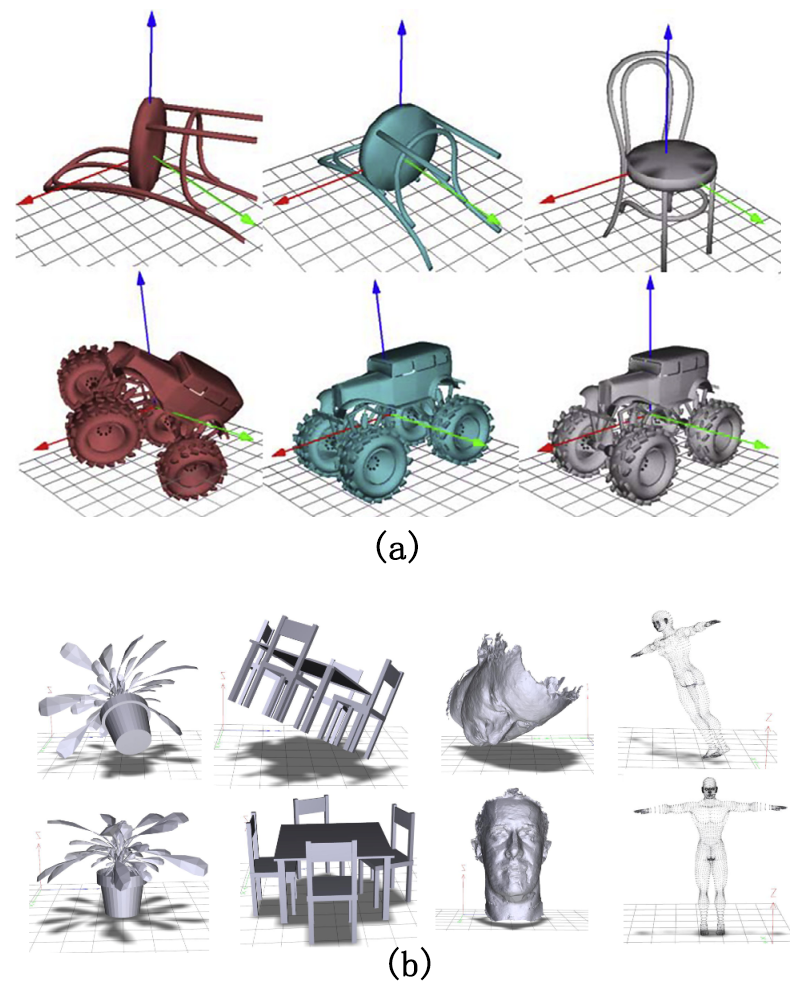
\includegraphics[width=3in]{images/upright_lowrank}
  \caption{Low rank: unsupervised upright orientation. (a): local method\cite{jin2012unsupervised}. (b): global method\cite{wang2014upright}.}
\end{figure} 